% !TeX root = ../../main.tex
室内冲砂实验表明，对于连续砂床或严重出砂井况，常规水力冲砂效率低、除砂效果差：提高来流雷诺数虽可降低砂床的最大堆积高度，但砂头的无量纲运移速度始终低于4.0\%，砂床仍在砂头后方富集抬升，拖动管柱时砂卡风险甚至高于冲砂前，而排量又受设备输出能力的限制。实验还提示，砂床的“锁死”状态是制约冲砂效率的症结，若能持续改变来流的冲砂方向、破坏砂床的锁死条件，冲砂效率仍有提升空间。为此，本节将脉冲射流破床、旋转喷头全向冲洗与机械刮削、毛刷刷洗集成于一趟管柱，设计“三合一”脉冲式冲刮刷集成式井筒清洁工具，在阐明其结构组成与工作原理的基础上，依次开展关键单元的设计计算与校核、脉冲发生模块的动力学建模以及携砂与流场仿真，并结合整机技术参数、适用井况与管柱组合确定施工工艺，最后给出拆装维护规程与样机试验结果。

\subsection{水力脉冲冲砂洗井工具结构组成}
\label{subsec:structure_3_in_1}
水力脉冲冲砂洗井工具主要由脉冲发生器、旋转喷头、液压刮管器和毛刷刮管器构成，如图\ref{fig:tool_structure_3_in_1}所示。
脉冲发生器产生一种具有低频特性的高、负压交替水力冲击波。该模块通过对套管内壁进行高频次的反复激励，利用压力脉动产生的振动效应有效疏通并剥离附着于管壁的坚硬垢层与残留杂质。更为关键的是，水力冲击波在环空流体中传播时，能为已沉积或趋于沉积的砂砾提供额外的扰动动能，破坏颗粒间的动力平衡状态，从而显著提升井筒清砂的整体作业效率。
旋转喷头的核心功能是利用前向及后向布置的喷嘴产生强力射流，直接作用于井筒中或筛管内的沉积砂床，通过流体的高剪切应力实现对砂床表面的破坏与砂砾的卷扬，使沉积颗粒在卷扬作用下重新进入悬浮运移状态；同时，配合旋转机构实现周向全覆盖喷射，消除了常规清洗中的水力死角。
液压刮管器和毛刷刮管器则实现对套管内壁进行基于机械方法的深度清洁。

与现有的工具相比，所设计的“三合一”脉冲式冲刮刷集成式井筒清洁工具在功能上实现了水力冲砂、机械刮削和刷洗清洁的有机结合，能够在单次下入作业中完成对井筒内砂砾、铁屑、结垢物及蜡等杂质的高效清除，显著提升了井筒清洁的整体效率与效果。
\begin{figure}[htbp]
	\centering
	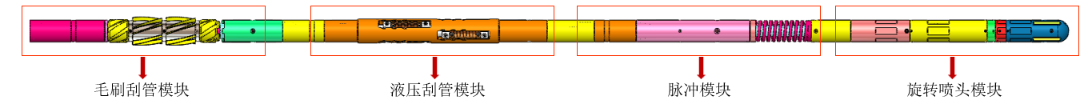
\includegraphics[width=1.0\textwidth]{figure/chapter3/tool-allstru-show.png}
	\caption{水力脉冲冲砂洗井工具结构示意图}
	\label{fig:tool_structure_3_in_1}
\end{figure}


\begin{figure}[htbp]
	\centering
	\subfloat[左段]{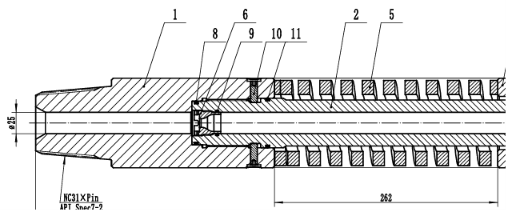
\includegraphics[width=\textwidth]{figure/chapter3/water-pressure-work.png}}\\[2pt]
	\subfloat[右段]{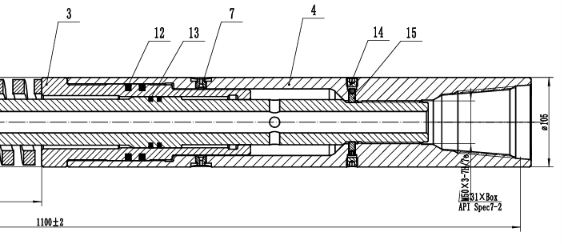
\includegraphics[width=\textwidth]{figure/chapter3/water-pressure-work-right.png}}
	\caption{MCQ105 脉冲器二维装配图（纵剖主视图，比例 1:5）}
	\label{fig:dwg-3in1}
\end{figure}

\subsection{水力脉冲冲砂洗井工具结构设计及工作原理}

\subsubsection{脉冲发生器}
如图\ref{fig:pulse_module}所示，脉冲发生器由上接头、心轴、移动活塞、矩形弹簧、下接头组成，其工作原理如图\ref{fig:principle_of_pulsing_tool}所示，工具的技术参数如表\ref{tab:pulsar_params}所示。脉冲发生模块圆周上设有出水孔，通过地面泵或注水管线将液体泵入井下，水流经节流喷嘴时产生节流压差，对脉冲器活塞端面形成高压作用。在高压作用下，活塞克服矩形弹簧的预紧力及流体的粘滞与摩擦阻力产生轴向位移，当活塞上端面到达侧向出水孔时，侧向出水孔开启，高压水射流从侧向出水孔喷出，腔内压力开始下降；活塞在弹簧压缩力的作用下开始复位，侧向出水孔关闭。活塞复位到初始位置后，系统开始下一循环。
\begin{figure}[htbp]
	\centering
	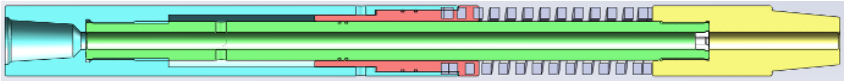
\includegraphics[width=.9\textwidth]{figure/chapter3/pulse-module.png}
	\caption{水力脉冲冲砂洗井工具脉冲发生器结构图}
	\label{fig:pulse_module}
\end{figure}

该装置向井筒环空传递振动能量的途径主要包括两种机制：一是脉冲器本体产生的轴向机械振荡；二是由高压脉冲流体激发的径向水力冲击效应。在上述复合动载荷的共同叠加下，环空内的局部流场呈现出强烈的瞬态扰动特性。原本压实沉积的砂床结构被脉冲射流破坏，砂粒由静态沉降转变为悬浮流化状态，进而配合循环工作液被高效排出井筒。
\begin{figure}[htbp]
	\centering
	\subfloat[脉冲发生模块蓄能阶段]{%
	\includegraphics[width=0.9\textwidth]{figure/chapter3/energy-storage-in-pulse-module.jpg}
	}
	\vspace{-0.5em}
	\subfloat[脉冲发生模块复位阶段]{%
	\includegraphics[width=0.9\textwidth]{figure/chapter3/restore-in-pulse-module.jpg}
	}
	\caption{脉冲发生器工作原理}
	\label{fig:principle_of_pulsing_tool}
\end{figure}

\begin{table}[htbp]
    \centering
    \caption{脉冲发生器技术参数}
    \label{tab:pulsar_params}
    \renewcommand{\arraystretch}{1.} % 增加行高，使表格更美观
    \begin{tabularx}{1.0\textwidth}{CCCCCCCC}
        \toprule % 顶线
        代号 & 适用套管规格 & \begin{tabular}[c]{@{}c@{}}组装外径\\ (mm)\end{tabular} & \begin{tabular}[c]{@{}c@{}}最小通径\\ (mm)\end{tabular} & \begin{tabular}[c]{@{}c@{}}长度\\ (mm)\end{tabular} & \begin{tabular}[c]{@{}c@{}}最大抗拉\\ (kN)\end{tabular} & \begin{tabular}[c]{@{}c@{}}最大抗扭\\ ($\text{kN}\cdot\text{m}$)\end{tabular} & 连接螺纹 \\
        \midrule % 栏目线
        MSQ105 & 4-1/2\inch & 105 & 25 & 1250 & 912 & 14.2 & \begin{tabular}[c]{@{}c@{}}NC31\\ ($\text{P}\times\text{B}$)\end{tabular} \\
        \bottomrule % 底线
    \end{tabularx}
\end{table}

\subsubsection{旋转喷头}
如图\ref{fig:nozzle_sub}所示，旋转喷头主要由上接头、筒体、心轴、连通隔套、平衡活塞、底部帽、平衡活塞座、喷头连接体、隔套、座、旋转喷头、喷嘴和骨架油封等密封件以及轴承和复位弹簧等零部件组成，其技术参数如表\ref{tab:rotary_nozzle_params}所示。旋转喷头位于工具作业串的最前端，由钻杆送入至指定位置。开泵循环泵入介质时，流体由工具上接头导入，沿中心心轴流道行进，最终经由端部喷嘴高速喷出形成射流。此外，为实现全向清洗，喷头结构中设计了若干具有特定偏心夹角的喷嘴。当高速介质经由倾斜流道射出时，射流产生的反冲推力在工具横截面上形成持续的偏心力矩，该力矩直接驱动旋转喷头与心轴自转，进而实现对套管内壁周向无死角清洗。
\begin{figure}[htbp]
	\centering
	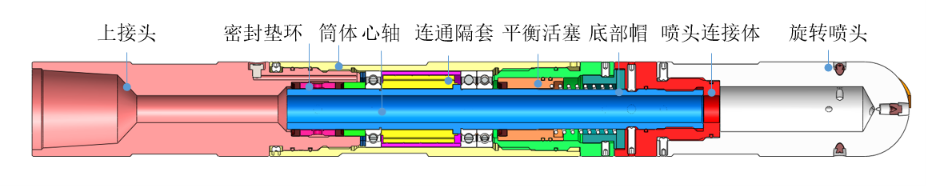
\includegraphics[width=1.0\textwidth]{figure/chapter3/roll-head.png}
	\caption{旋转喷头模块结构示意图}
	\label{fig:nozzle_sub}
\end{figure}

\begin{table}[htbp]
    \centering
    \caption{旋转喷头技术参数}
    \label{tab:rotary_nozzle_params}
    \renewcommand{\arraystretch}{1.} % 增加行高，使表格更美观
    \small % 9 列较宽，用小一号字避免超出页边距
    \setlength{\tabcolsep}{3pt}
    \begin{tabularx}{1.0\textwidth}{CCCCCCCCC}
        \toprule % 顶线
        \begin{tabular}[c]{@{}c@{}}外径\\ (mm)\end{tabular} & 
        \begin{tabular}[c]{@{}c@{}}总长\\ (mm)\end{tabular} & 
        \begin{tabular}[c]{@{}c@{}}喷嘴尺寸\\ (mm $\times$ n)\end{tabular} & 
        \begin{tabular}[c]{@{}c@{}}工作排量\\ (L/min)\end{tabular} & 
        \begin{tabular}[c]{@{}c@{}}转速\\ (r/min)\end{tabular} & 
        \begin{tabular}[c]{@{}c@{}}工作压强\\ (MPa)\end{tabular} & 
        扣型 & 
        \begin{tabular}[c]{@{}c@{}}最大抗拉\\ (kN)\end{tabular} & 
        \begin{tabular}[c]{@{}c@{}}最大抗扭\\ ($\text{kN}\cdot\text{m}$)\end{tabular} \\
        \midrule % 栏目线
        105 & 1045 & $3.175 \times 7$ & $100\sim500$ & $10\sim300$ & $\le 70$ & \begin{tabular}[c]{@{}c@{}}NC31\\ ($\text{P}\times\text{B}$)\end{tabular} & 663 & 8.5 \\
        \bottomrule % 底线
    \end{tabularx}
    \par\vspace{4pt}{\small 注：表中最大抗拉、最大抗扭为按危险截面计算的承载能力，其数值高于图纸技术要求规定的许用拉力 $400\,\mathrm{kN}$、许用扭矩 $8\,\mathrm{kN\cdot m}$（后者为设计指标，见表\ref{tab:pulsar_design_req}），二者含义不同。}
\end{table}

\subsubsection{毛刷刮管器}
MSQ型毛刷刮管器主要由上接头、上扶正套、毛刷体、下扶正套、剪切套、剪切定位套、下接头等部件组成。工作时，主要依靠上、下毛刷对刮削后的套管内壁进行刷洗清洁。毛刷刷丝为挠性元件，当刷丝端部产生磨损时，刷丝可回弹补偿，从而保证整个作业过程中对套管产生持续的清洁。刷丝采用回弹性能好、硬度高、耐磨损、耐腐蚀的$304$不锈钢丝，直径$\phi 0.2\mathrm{mm}$，外伸长度$15\mathrm{mm}$，刷里由不锈钢冲压成形，机械夹紧刷丝。毛刷体上开有燕尾槽，刷里镶嵌在燕尾槽内，刷里与毛刷体之间通过燕尾槽的啮合实现自锁，从而保证刷里在作业过程中不会脱落。毛刷刮管器的结构如图\ref{fig:swiper_in_3_in_1}所示，技术参数如表\ref{tab:brush_scraper_params}所示。
\begin{figure}[htbp]
	\centering
	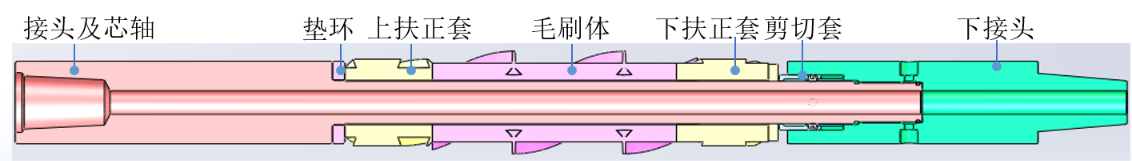
\includegraphics[width=0.9\textwidth]{figure/chapter3/water-pluse.png}
	\caption{毛刷刮管器结构简图}
	\label{fig:swiper_in_3_in_1}
\end{figure}

\begin{table}[htbp]
    \centering
    \caption{毛刷刮管器技术参数}
    \label{tab:brush_scraper_params}
    \renewcommand{\arraystretch}{1.} % 增加行高，使表格更美观
    \begin{tabularx}{1.0\textwidth}{CCCCCC}
        \toprule % 顶线
        型号 & 
        \begin{tabular}[c]{@{}c@{}}最大外径\\ (mm)\end{tabular} & 
        \begin{tabular}[c]{@{}c@{}}毛刷最大外径\\ (mm)\end{tabular} & 
        \begin{tabular}[c]{@{}c@{}}水眼\\ (mm)\end{tabular} & 
        \begin{tabular}[c]{@{}c@{}}总长\\ (mm)\end{tabular} & 
        接头扣 \\
        \midrule % 栏目线
        MSQ54 & 105 & 130 & 20 & 1250 & NC31($\text{P}\times\text{B}$) \\
        \bottomrule % 底线
    \end{tabularx}
\end{table}

\subsubsection{液压刮管器}
液压刮管器的主要用途是清除井下套管内壁的水泥、沉积蜡、射孔飞边以及其他附着物，保证套管内壁的清洁，以利所有钻井工具的正常作业。液压刮管器主要有上接头、筒体、连接体、下接头、芯轴、刮刀等部件组成，其结构如图\ref{fig:scrapper_in_3_in_1}所示，技术参数如表\ref{tab:hydraulic_scraper_params}所示。
\begin{figure}[htbp]
	\centering
	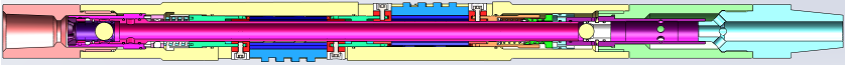
\includegraphics[width=0.9\textwidth]{figure/chapter3/scraper-in-3-in-1.png}
	\caption{液压刮管器结构简图}
	\label{fig:scrapper_in_3_in_1}
\end{figure}

\begin{table}[htbp]
    \centering
    \caption{液压刮管器技术参数}
    \label{tab:hydraulic_scraper_params}
    \renewcommand{\arraystretch}{1.} % 增加行高，使表格更美观
    \small % 7 列较宽，用小一号字避免超出页边距
    \setlength{\tabcolsep}{3pt}
    \begin{tabularx}{1.0\textwidth}{CCCCCCC}
        \toprule % 顶线
        代号 & 适用套管规格 & \begin{tabular}[c]{@{}c@{}}组装外径\\ (mm)\end{tabular} & \begin{tabular}[c]{@{}c@{}}最小通径\\ (mm)\end{tabular} & \begin{tabular}[c]{@{}c@{}}投入钢球\\ (mm)\end{tabular} & \begin{tabular}[c]{@{}c@{}}张开直径\\ (mm)\end{tabular} & 连接螺纹 \\
        \midrule % 栏目线
        YYGG105 & 4-1/2\inch & 114 & 22 & 28/32 & 130 & NC31($\text{P}\times\text{B}$) \\
        \bottomrule % 底线
    \end{tabularx}
\end{table}

所设计的液压刮管器创新之处在于刮刀可复位。刮刀采用投球的方式激活，投入$\mathrm{S}\phi 28$的钢球打压剪切限位销钉后，泵入的大流量洗井液形成节流压差，反向推动活塞，进而驱动刮刀沿径向斜槽张开。张开后的刮刀最大外径可达130mm，可清洁 5-1/2\inch 套管。张开的刮刀会被心轴上的分瓣螺纹锚定机构锁定，保证了刮削过程中的稳定。如果在刮削过程中出现卡钻的情况，可投$\mathrm{S}\phi 32$的钢球激活刮刀复位机构，打压收回刮刀，从而实现工具防卡。

在工具的通过性方面，刚性结构件的最大外径是$105\mathrm{mm}$，比内径为4.75\inch （120.65 mm）的密封筒直径小$15.65\mathrm{mm}$，保证了工具在井下的顺利通过。对于现场使用的公称尺寸为5-1/2\inch 的筛管和盲管，内径为$4.825\inch$（122.56mm），工具比筛管和盲管的内径小$17.56\mathrm{mm}$，保证了工具在筛、盲管中的通过性。
